\chapter{Identification of transfer function of a Single Board Heater System through Ramp response experiments}
The Aim of this experiment is to perform Ramp test on the Single Board Heater System and to identify the system transfer function using Ramp response data. The target group is anyone who has basic knowledge of Control Engineering.
\section{About this Experiment}

\begin{figure}
\centering
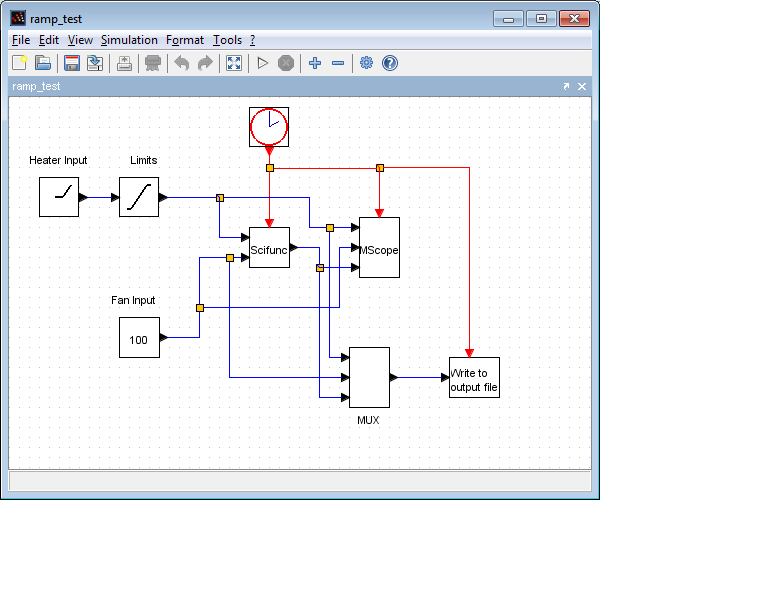
\includegraphics[width=0.7\linewidth]{Ramp-test_manual/ramp_xcos.jpg}
\caption{Xcos for Ramp Test experiment}
\label{Xcos_rt}
\end{figure} 
We have used Scilab-5.2.2 and Xcos for sending and receiving data. This interface is shown in Fig.\ref{Xcos_rt}. Heater current and fan speed are the two inputs to the SBHS system. They are given in PWM units. These inputs can be varied through the Xcos interface by setting the properties of the input blocks in Xcos. The data acquired in the process is stored in the local drive using the "Write to output file" block and is available to the user for further analysis.
\section{Theory}
Identification of the transfer function of a system is quite important since it helps us to model the physical system mathematically. Once the transfer function is obtained one can find out the response of the system, to various inputs, without actually applying them to the system.
Consider the standard first order transfer function given below
\begin{align}
G(s) &= \frac{ C(s)}{ R(s)}\\
G(s)&=\frac K{\tau s+1}\\                           
\intertext{Rewriting the equation by substituting equation 4.2 in equation 4.1, we get}
C(s)  &= K \left\{\frac {R(s)}{\tau s + 1}\right\}\label{fotf}
\intertext{Let us consider the case of giving a ramp input to this first order system. The Laplace Transform of a ramp function with slope = $\upsilonup$ is $ \frac \upsilonup {s^2}$. Substituting $ R(s) = \frac \upsilonup {s^2}$ in equation \ref{fotf}, we obtain}
C(s) & =  \frac K{\tau s + 1}\frac \upsilonup {s^2}\\
&= \frac A{s} + \frac B{s^2} +\frac C{\tau s + 1}\\
\intertext{Solving $C(s)$ using Heaviside expansion approach, we get}
C(s) &= K\upsilonup \left\{\frac1{s^2} -  \frac \tau s + \frac {\tau^2}{\tau s + 1}\right\}\label{Heaviside}\\
\intertext{Taking the Inverse Laplace transform of the above equation, we get}
c(t)&= K\upsilonup \left\{t -\tau   + \tau e^{\frac {-t}\tau }\right\}\label{ct} \\
\intertext{The difference between the reference and output signal is the error signal $e(t)$. Therefore,}
e(t)&= r(t) - c(t)\\
e(t)&= K\upsilonup t - K\upsilonup t + K\upsilonup \tau  - K\upsilonup \tau e^\frac {-t}\tau   \\
e(t)&= K\upsilonup \tau (1 - e^{\frac {-t}\tau})\label{et}\\
\intertext{Normalizing equation \ref{et} for $t>>\tau$, we get}
e(t) &= \tau
\end{align}
This means that the error in following the ramp input is equal to $\tau$ for large value of $t$ \cite{ogt05}. Hence, the smaller the time constant $\tau$ , the smaller is the steady state error.
\section{Step by step procedure to perform Ramp Test}
Change the scilab working directory to {\tt Ramp\_Test} folder. Execute the code {\tt ser\_init.sce} and {\tt ramp\_test.sci}. Open the Xcos code {\tt ramp\_test.xcos}. Give a ramp input to the system with some value for slope. For this experiment, we have chosen $slope = 0.1$. Double click on the ramp input block labled as "Heater input". Put the following values in the respective fields. Slope = 0.1, start time = 300, initial output = 20. Keep the fan constant at 100. Note that the value of heater current will not exceed 40 PWM units due to the use of limit blocks. Running the xcos code may warn you with a message saying "No continuous-time states. Thresholds are ignored". Ignore the message by clicking on OK button.
\begin{figure}
\centering
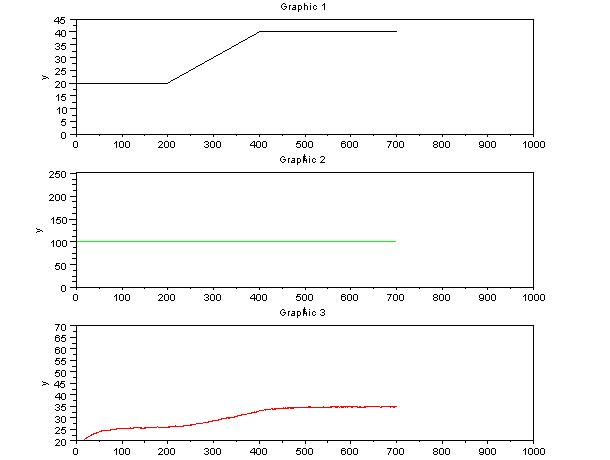
\includegraphics[width=\linewidth]{Ramp-test_manual/ramp_plot.jpg}
\caption{Screen shot of Ramp Test Experiment}
\end{figure}
The data thus obtained is stored using "Write to output file" Xcos block as shown in Fig.\ref{Xcos_rt}.
\begin{table}
\begin{verbatim}
 0.000E+00  0.100E+02  0.100E+03  0.216E+02
 0.100E+00  0.100E+02  0.100E+03  0.216E+02
.
.
 0.251E+03  0.300E+02  0.100E+03  0.291E+02
 0.251E+03  0.300E+02  0.100E+03  0.291E+02
\end{verbatim}
\caption{Ramp data obtained after performing the Ramp Test}
\label{Rampdata}
\end{table}
The first column of Table \ref{Rampdata} denotes time in seconds. The second column denotes heater current. The third column denotes the fan speed. It has been held constant at 100 units. The last column denotes the plate temperature.
\\
\section{Ramp Analysis}
After completing the ramp test experiment, let us do the analysis. Change the directory to {\tt Ramp\_Analysis}. Execute the file {\tt ramp.sce}. On executing this file, you get the values of Kp, tau and Kp approx and tau approx on the Scilab Console Window. You will also get a plot of the ramp response calculated using the equation \ref{ct} for Kp and tau values.
\begin{figure}[h]
	\centering
		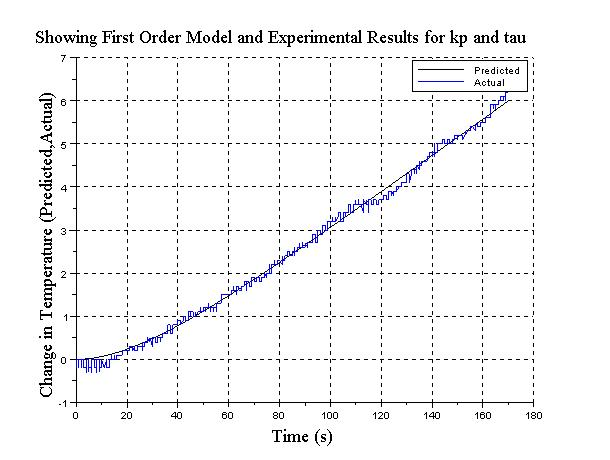
\includegraphics[width=\linewidth]{Ramp-test_manual/fit_curve_ramp.jpg}
	\caption{Ramp response for Kp and tau}
	\label{fig:fit_curve_ramp}
\end{figure}

\section{Discussion}
We summarize our findings now. The experiment has been performed by varying the heater current and keeping the fan speed constant. However, the user is encouraged to try out the experiment using different combinations of fan speed and heater current. Negative ramp can also be tried out to make the experiment more informative. It is not necessary to keep a particular input constant. For example, you can try giving a step input to the disturbance signal, i.e., the fan input. The system can also be treated as a second order system. This consideration is necessary since it increases the accuracy of the acquired transfer function.\cite{kmm09}
\section{Conducting Ramp Test on SBHS, virtually}
The step by step procedure for conducting an experiment virtually is explained in section \ref{vlabsexpt}. The required .sce file is {\tt ramptest.sce}.  You will find this file in the {\tt RampTest} directory under {\tt virtual} folder. Please note that the analysis code of ramp test data obtained by a virtual experiment is slightly different. The procedure to use the analysis code however remains the same as explained earlier. To do a first order analysis, one has to use the file {\tt firstorder\_virtual.sce}. These files are available in the {\tt Ramp\_Analysis} folder under the {\tt virtual} folder. The necessary codes are listed in the section \ref{rampcodes}.

\section{Scilab Code}\label{rampcodes}
\begin{code}
\ccaption{ramp\_test.sci}{\ttfamily ramp\_test.sci}
\lstinputlisting{Scilab/local/Ramp_Test/ramp_test.sci}
\end{code}

\begin{code}
\ccaption{label.sci}{\ttfamily label.sci}
\lstinputlisting{Scilab/local/Ramp_Analysis/label.sci}
\end{code}

\begin{code}
\ccaption{cost.sci}{\ttfamily cost.sci}
\lstinputlisting{Scilab/local/Ramp_Analysis/cost.sci}
\end{code}

\begin{code}
\ccaption{cost\_approx.sci}{\ttfamily cost\_approx.sci}
\lstinputlisting{Scilab/local/Ramp_Analysis/cost_approx.sci}
\end{code}

\begin{code}
\ccaption{ramptest.sci}{\ttfamily ramptest.sci}
\lstinputlisting{Scilab/virtual/RampTest/ramptest.sci}
\end{code}

\begin{code}
\ccaption{ramptest.sce}{\ttfamily ramptest.sce}
\lstinputlisting{Scilab/virtual/RampTest/ramptest.sce}
\end{code}

\begin{code}
\ccaption{ramp\_virtual.sce}{\ttfamily ramp\_virtual.sce}
\lstinputlisting{Scilab/virtual/Ramp_Analysis/ramp_virtual.sce}
\end{code}


%\bibliography{New} % Adding References
